\section{Practical Application of PCA [5pts]}
This question will ask about the application of PCA onto the dataset used in section 2 of the Programming assignment. While that section may be helpful, this question is standalone.

\begin{enumerate}[label=\alph*.]
    \item After applying PCA to the wine dataset, we can analyze what proportion of total variance is expressed by each component. By the nature of the algorithm, they actually already come sorted by how much variance they express. Usually, we keep the top N most expressive components, and we can add up the variance they capture for a cumulative graph. We can plot this for our 13-dimensional wine dataset.
    \begin{figure}[h]
        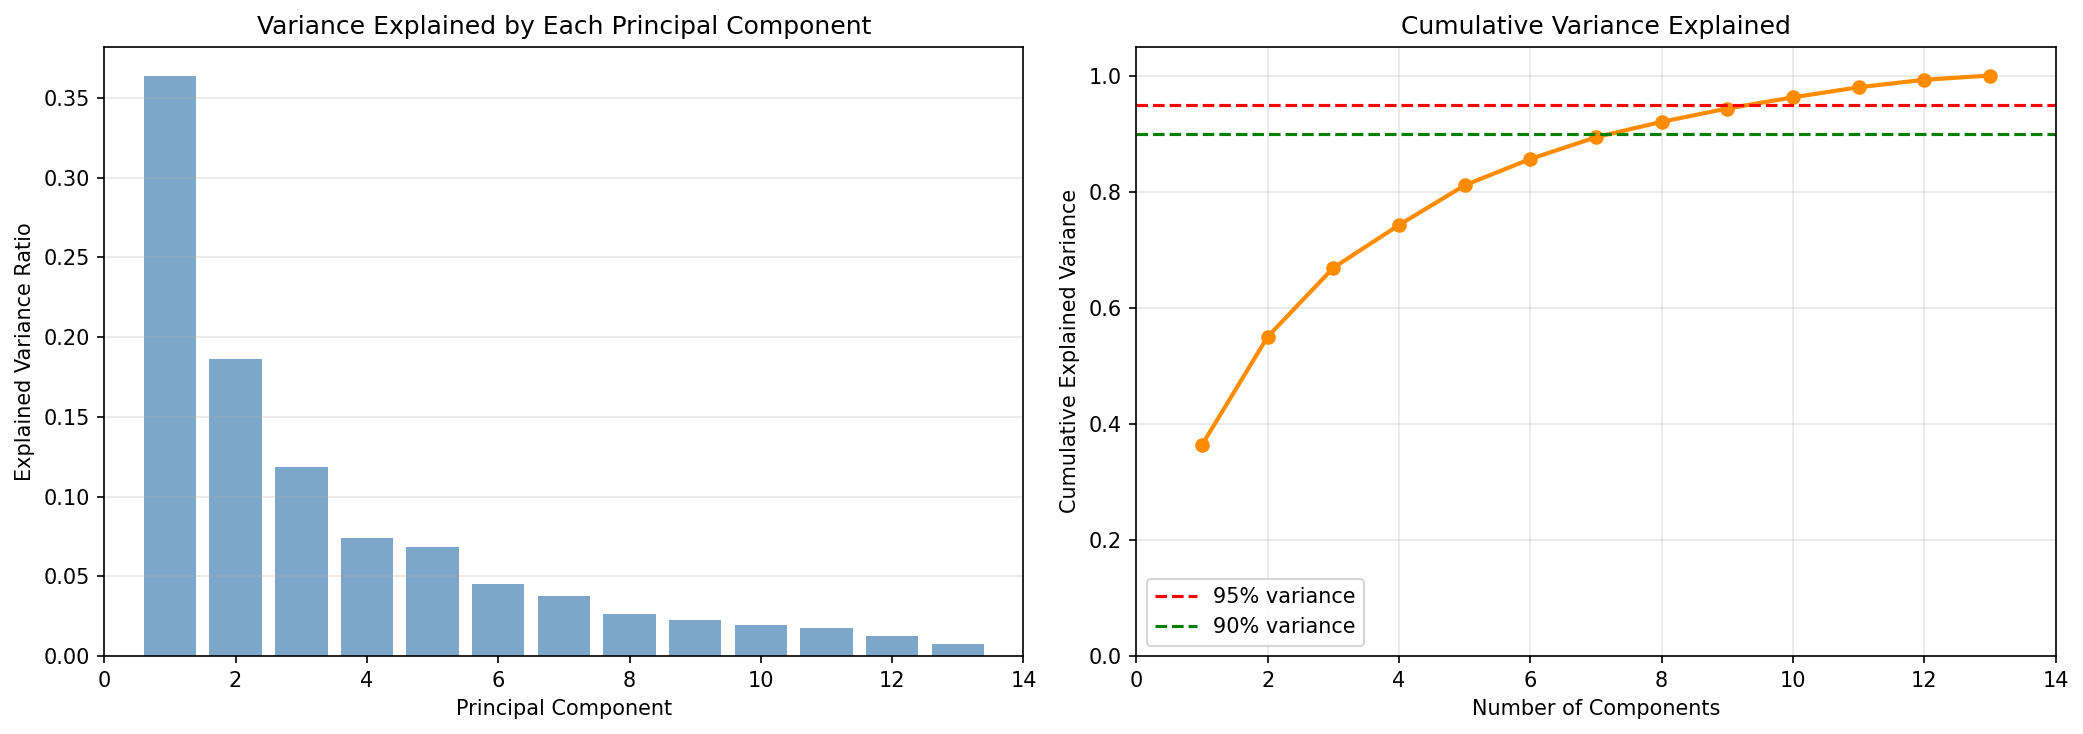
\includegraphics[width=\textwidth]{questions/images/Q2-explained-variance.png}
        \caption{Left: the variance of each component, Right: the cumulative variance of the top N components together}
        \label{fig:Q2-fig}
    \end{figure}

    Based on the cumulative variance plot above, what is the minimum number of principal components required to capture 95\% of the total variance? What does this tell you about the redundancy in the original 13 features? [2pts]

    \item PCA can be thought of as a projection onto a set of basis vectors that follow the directions of maximum variance in the data. PCA, then, is often a useful preprocessing step for classification models that perform simple inferences or computations on the features themselves, e.g., a decision tree, which repeatedly splits the dataset along individual features.

    While it \textit{often} does improve classification performance, PCA isn't \textit{guaranteed} to do so. Why might choosing axes that maximize variance not necessarily improve class separability along the axes? [3pts]

\end{enumerate}